%----------------------------------------------------------------------------
\chapter{TPSC specifikációk vizualizációja}
%----------------------------------------------------------------------------

A specifikációk vizualizációjához a \textit{Modell alapú rendszertervezés} tárgy során készített PSC vizualizációs Sirius alkalmazást használtam fel.
Előszőr kiegészítettem az alkalmazást TPSC elemek vizualizációjával.
Egy \textit{XML} generátor előállítja a specifikáció \textit{XMLs} leírását, amit a Sirius alkalmazás képes feldolgozni és előállítani a hozzá tartozó diagramot.

\begin{figure}[!ht]
    \centering
    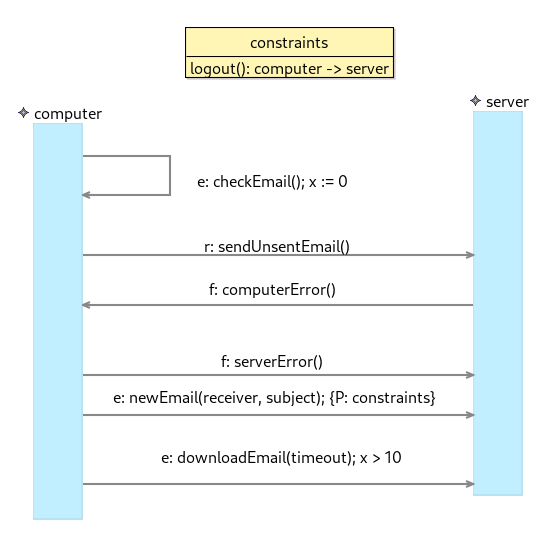
\includegraphics[width=150mm, keepaspectratio]{figures/diagramExample.png}
    \caption{Szenárió diagram.}
\end{figure}

\begin{lstlisting}[language=java, frame=single, float=ht!, caption={Szenárió diagram xml leírása.},captionpos=b]
<?xml version="1.0" encoding="UTF-8"?>
<minotor:SequenceDiagram xmi:version="2.0" xmlns:xmi="http://www.omg.org/XMI" xmlns:minotor="hu.bme.mit.mdsd.xboyz.erdiagram" Name="Email">

<lifelines Name="computer" Type="Computer"/>
<lifelines Name="server" Type="Server"/>

<constraints Name="constraints">
<transitions Name="logout()" source="//@lifelines.0" target="//@lifelines.1"/>
</constraints>

<transitions Name="checkEmail()" Type="REGULAR" Label="e: checkEmail()" source="//@lifelines.0" target="//@lifelines.0"  after="//@transitions.1" reset="x"/>
<transitions Name="sendUnsentEmail()" Type="REQUIRED" Label="r: sendUnsentEmail()" source="//@lifelines.0" target="//@lifelines.1" before="//@transitions.0" after="//@transitions.2"/>
<transitions Name="computerError()" Type="FAIL" Label="f: computerError()" source="//@lifelines.1" target="//@lifelines.0" before="//@transitions.1" after="//@transitions.3"/>
<transitions Name="serverError()" Type="FAIL" Label="f: serverError()" source="//@lifelines.0" target="//@lifelines.1" before="//@transitions.2" after="//@transitions.4"/>
<transitions Name="newEmail(receiver, subject)" Type="REGULAR" Label="e: newEmail(receiver, subject)" source="//@lifelines.0" target="//@lifelines.1" before="//@transitions.3" after="//@transitions.5" constraint="//@constraints.0" constraintType="PAST"/>
<transitions Name="downloadEmail(timeout)" Type="REGULAR" Label="e: downloadEmail(timeout)" source="//@lifelines.0" target="//@lifelines.1" before="//@transitions.4"   clockConstraint="x &gt; 10"/>
</minotor:SequenceDiagram>
\end{lstlisting}

A diagramon az egyes objektumok kék \textit{lifeline} formájában jelenek meg.
Minden üzenethez tartozik egy nyíl.
A nyíl címkéjére írjuk az üzenet összes tulajdonságát.
A nyíl eleje és vége \textit{lifeline}-okat kötnek össze, amik az üzenet feladóját és fogadóját jelzik.
A megkötéseket egy sárga táblázat formájában reprezentáljuk, amelybe bele írjuk az összes megkötésben szereplő üzenetet.